\renewcommand{\theequation}{\theenumi}
\begin{enumerate}[label=\arabic*.,ref=\thesubsection.\theenumi]
\numberwithin{equation}{enumi}
\item let assume $P\left(X=1\right)$ be the probability of hitting 6 so
\begin{align}
\vec {P\left(X=1\right)} &= \frac{6}{30}
\\
&= \frac{1}{5}
\end{align}
$P\left(X=0\right)$ be the probability of not hitting the boundry
\begin{align}
P\left(X=0\right) &= 1 - P\left(A\right)
\\
&= 1-\frac{1}{5}
\\
&= \frac{4}{5}
\end{align}
codes for the above equation can be get from here
\begin{lstlisting}
codes/prob/prob1.py
\end{lstlisting}
\begin{figure}[!ht]
	\centering
	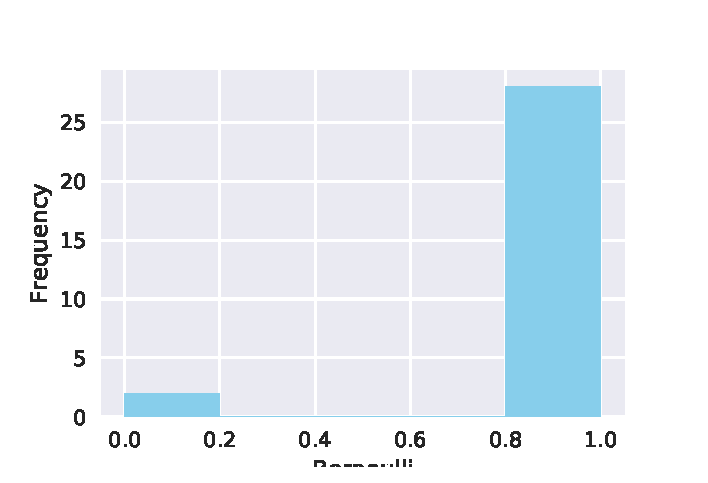
\includegraphics[width=\columnwidth]{./figures/prob/prob1.eps}
	\caption{bernoulli distribution1 }
	\label{fig:bt1}
	\begin{lstlisting}
	codes/prob/prob1.py
	\end{lstlisting}
\end{figure}
\end{enumerate}